% coding:utf-8

%----------------------------------------
%FOSADSVB, a LaTeX-Code for a summary of digital signal processing
%Copyright (C) 2015, Mario Felder & Michi Fallegger

%This program is free software; you can redistribute it and/or
%modify it under the terms of the GNU General Public License
%as published by the Free Software Foundation; either version 2
%of the License, or (at your option) any later version.

%This program is distributed in the hope that it will be useful,
%but WITHOUT ANY WARRANTY; without even the implied warranty of
%MERCHANTABILITY or FITNESS FOR A PARTICULAR PURPOSE.  See the
%GNU General Public License for more details.
%----------------------------------------

\chapter{Multirate und Filterbänke}
\section{Decimation}
Um ein Signal donwzusamplen, wird einfach nur jedes $D$te Sampel verwendet.
\begin{center}
	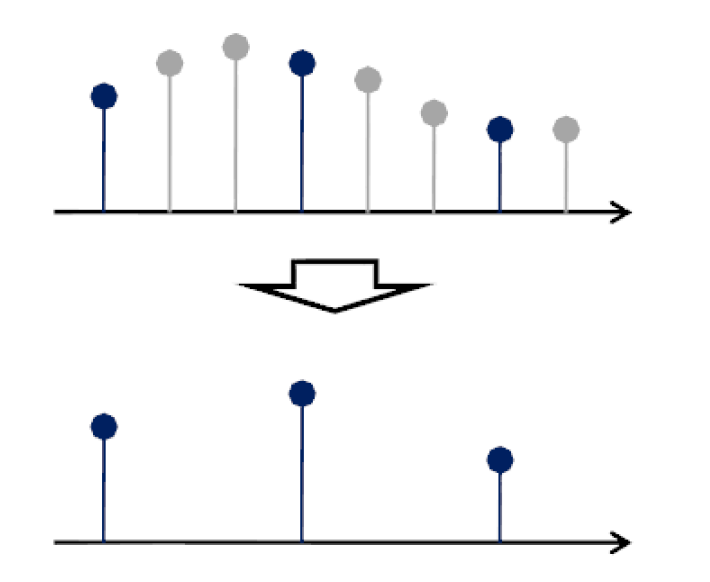
\includegraphics[scale=.7]{./images/downsample}
\end{center}
Dabei muss beachtet werden, dass das Abtasttheorem noch eingehalten wird. Das
Signal muss zuerst Tiefpass gefiltert werden. Die Frequenzantwort des TP ist
idealerweise:
\[ H(\Omega) = \left\lbrace \begin{matrix}
	1 & \textrm{if } \Omega \in [-\pi/D,\pi/D]\\
	0 & \textrm{otherwise}
\end{matrix} \right. \] 
\begin{center}
	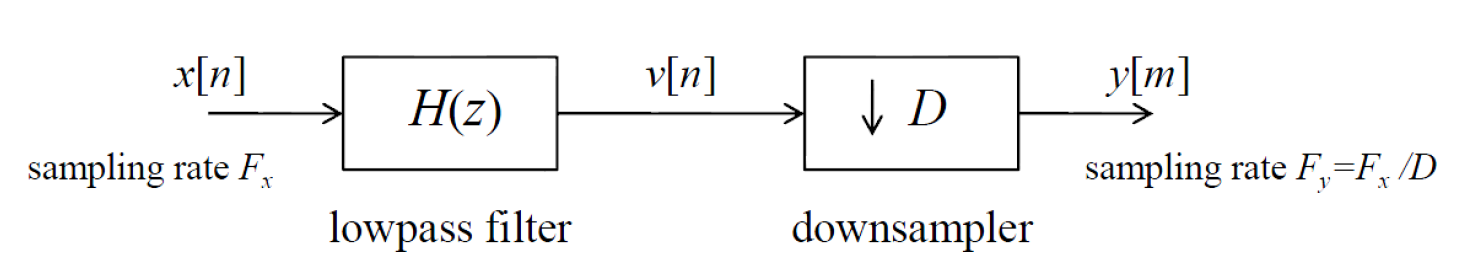
\includegraphics[scale=.7]{./images/decimation}
\end{center}
Das Resultat kann beschriben werden als $y[m] = v[mD]$. Das Frequenzspektrum
wird um den Faktor $D$ gespreizt. Für einen idealen TP-Filter gilt:
\[ Y(\Omega) = \frac{1}{D} V(\Omega/D)  \]
Allgemein:
\[ Y(\Omega) = \frac{1}{D} \sum_{d=0}^{D-1} V(\Omega/D-2\pi d/D) \]
\begin{center}
	\includegraphics[scale=.6]{./images/decimation_frequenz}
\end{center}
Als TP-Filter kann ein FIR Filter verwendet werden. Eine direkte Implementierung
ist nicht effektiv, da $D-1$ vom Filter berechnete Werte vom Downsampler
weggeworfen werden. Mit dem Downsampler vor dem Filter müssen weniger
Berechnungen durchgeführt werden.
\begin{center}
	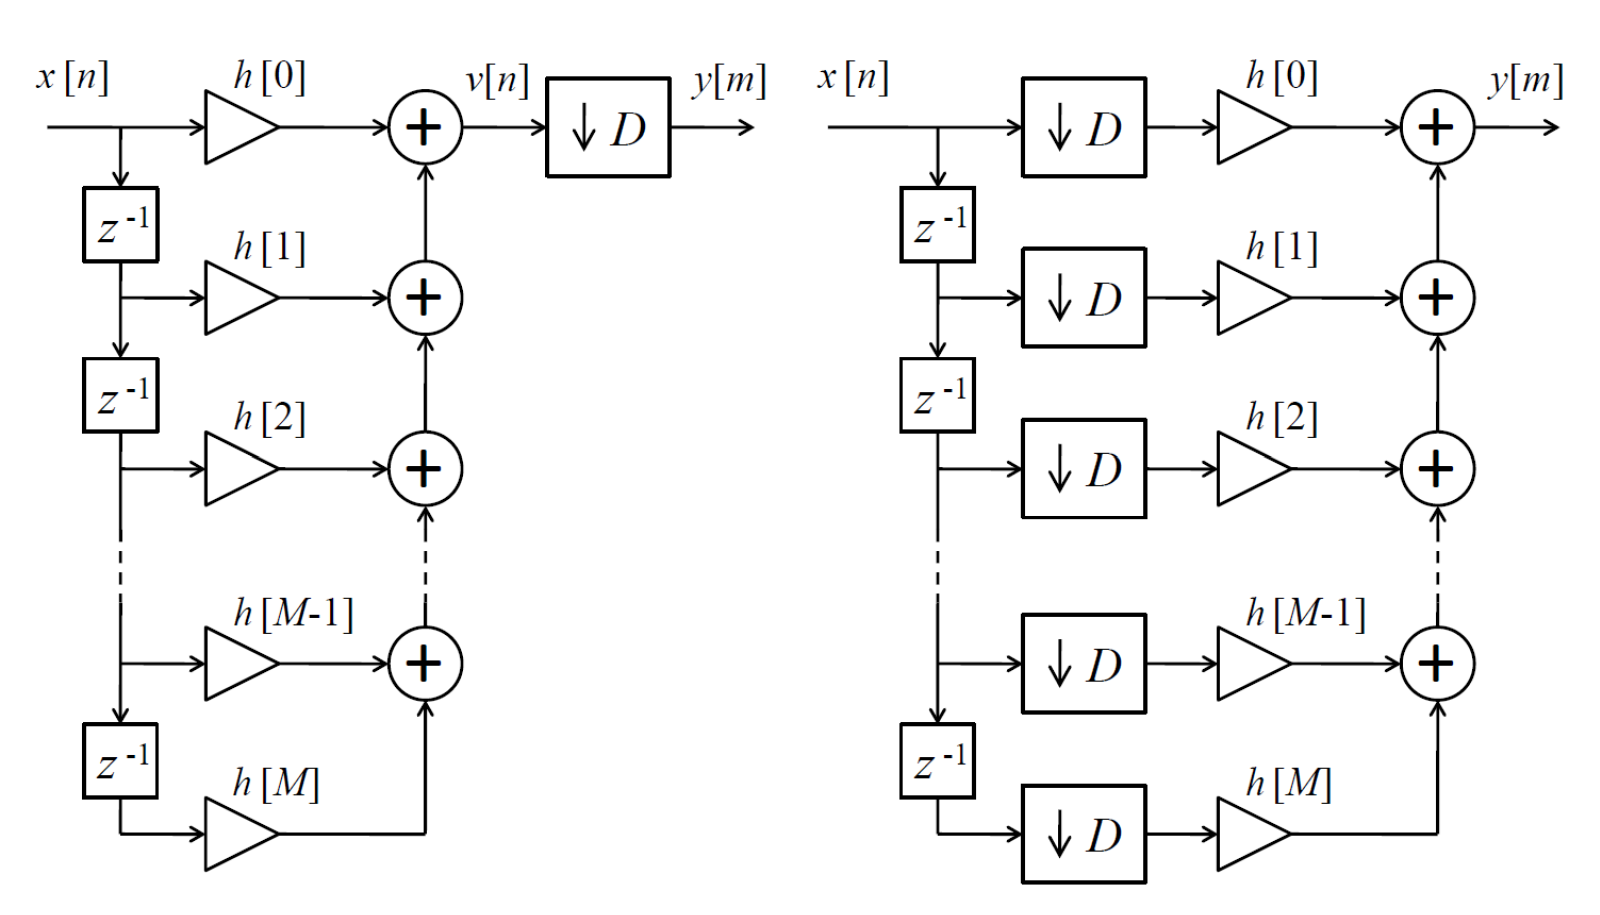
\includegraphics[scale=.7]{./images/decimation_scheme}
\end{center}

%===============================================================================
\section{Interpolation}
Bei einem Upsampler mit dem Faktor $I$ werden zwischen zwei Samples jeweils
$I-1$ Nullen eingefügt.
\begin{center}
	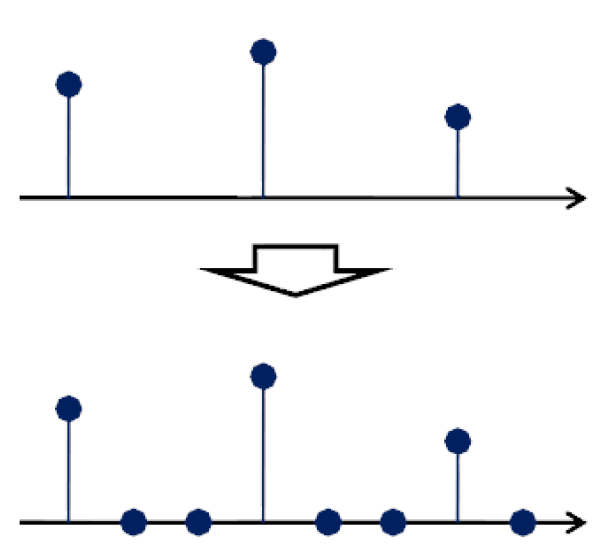
\includegraphics[scale=.7]{./images/upsample}
\end{center}
\[ r[n] = \left\lbrace \begin{matrix}
	y[n/I] & \textrm{if } n \in [0,\pm I, \pm 2I,\ldots]\\
	0 & \textrm{otherwise}
\end{matrix} \right. \] 
Die Abtastfrequenz $F_z$ ist $I$-mal höher als die Abtastfrequenz $F_y$ von
$y[m]$. Das Spektrum des upgesampelten Signal ist:
\[ \begin{aligned} R(\Omega) &= \sum_{n=-\infty}^{\infty} r[n]
	\e^{-\im\Omega n} \\
	&= \sum_{m=-\infty}^{\infty} r[m]\e^{-\im\Omega m}\\
	&= Y(I\Omega)  \end{aligned} \]
Damit das Frequenzspektrum von $y[m]$ nicht periodisch mit der Periode
von $2\pi/I$ ist, ist eine Tiefpassfilterung nach dem Upsampling notwendig. Der
ideale TP-Filter hat die Frequenzantwort:
\[ H(\Omega) = \left\lbrace \begin{matrix}
	I & \textrm{if } \Omega \in [-\pi/I,\pi/I]\\
	0 & \textrm{otherwise}
	\end{matrix} \right. \]
\begin{center}
	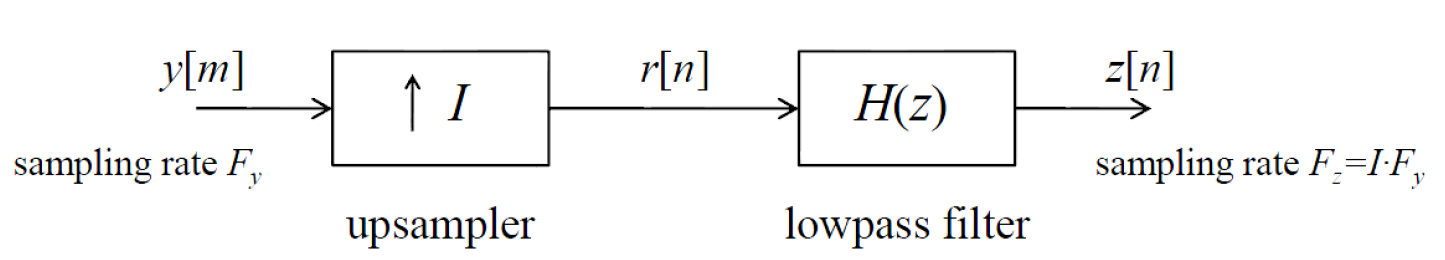
\includegraphics[scale=.7]{./images/interpolation}
\end{center}
\begin{center}
	\includegraphics[scale=.7]{./images/interpolation_frequenz}
\end{center}
Ein FIR oder IIR Filter kann als TP-Filter verwendet werden. Eine direkte
Implementierung ist ineffektiv, da der Filter auch auf die Null werte angewandt
wird.
\begin{center}
	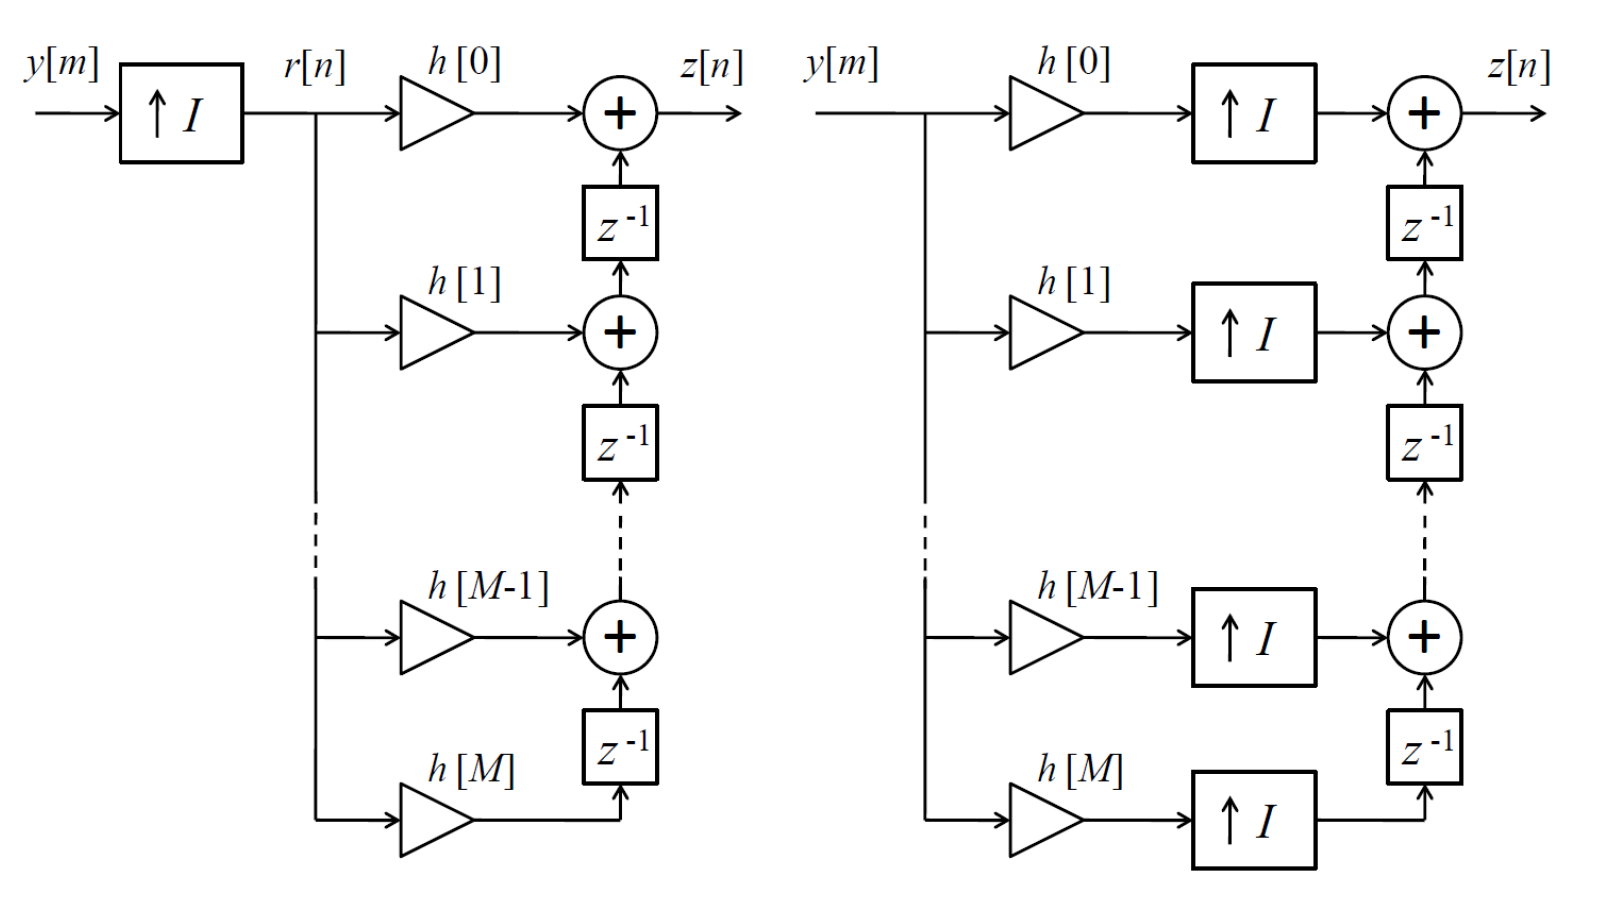
\includegraphics[scale=.7]{./images/interpolation_scheme}
\end{center}

%===============================================================================
\section{Polyphasen Filter}
Die um $M$ downgesampelte Impulsantwort $h[k]$ ist definiert als:
\[ p_i[k] = h[kM+i] \qquad i=0,1,\ldots,M-1 \]
Dazugehörende z-Transformation:
\[ P_i(z) = \sum_{k=-\infty}^{\infty} p_i[k]z^{-k} \qquad i0,1,\ldots,M-1 \]
Somit
\[ H(z) = \sum_{i=0}^{M-1}z^{-1} P_i(z^M) \]

\begin{minipage}{.48\textwidth}
	\centering
	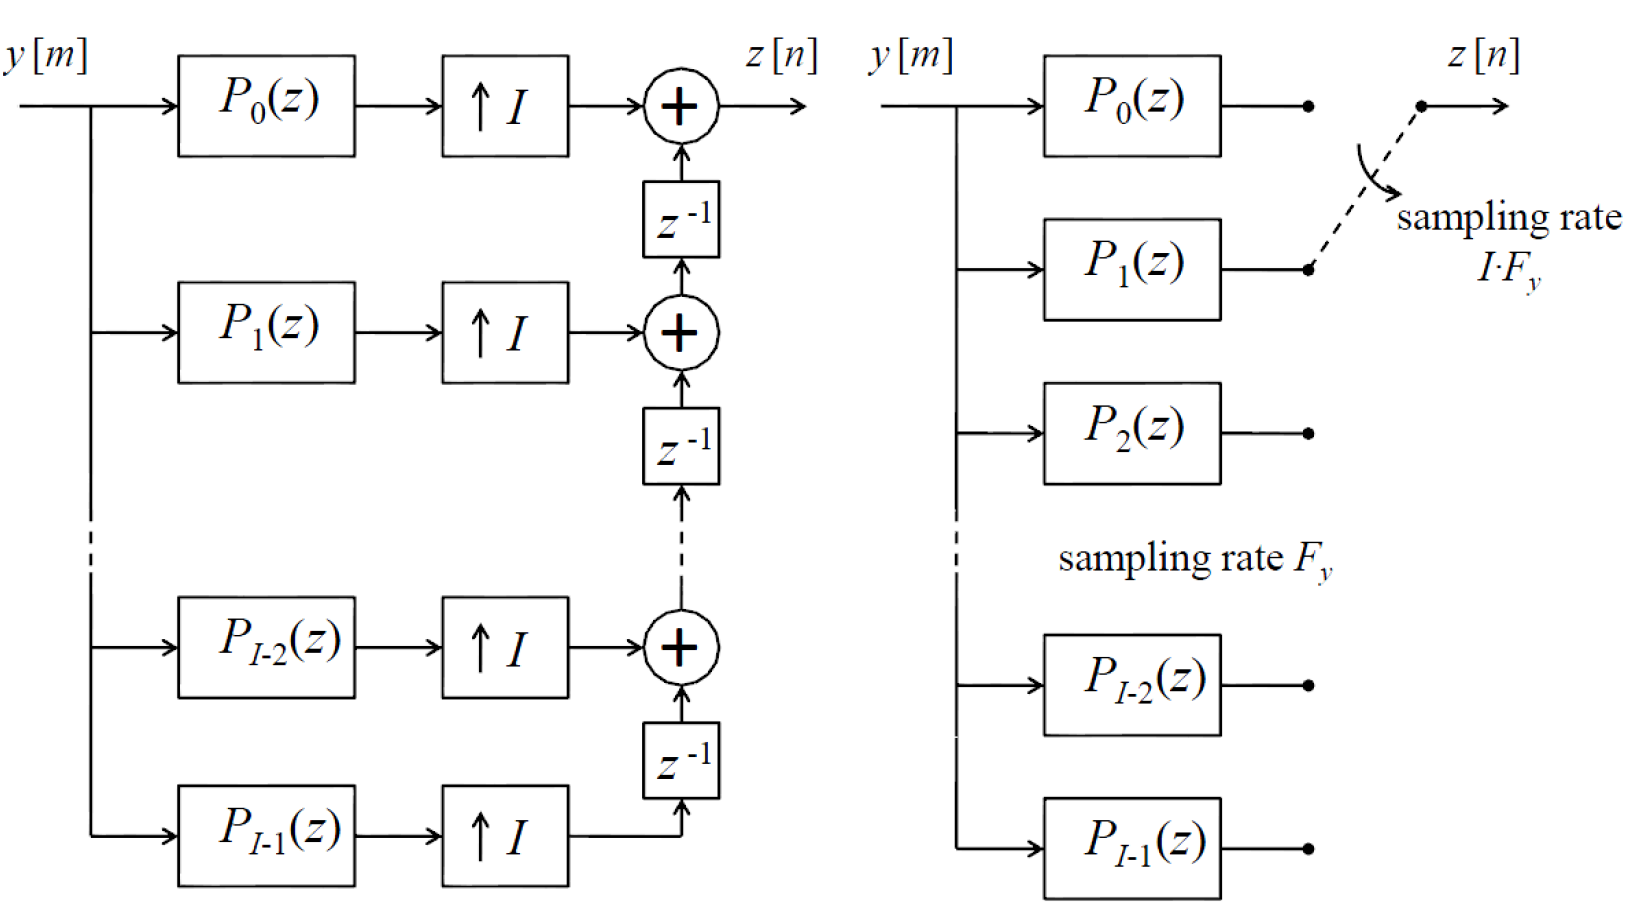
\includegraphics[width=\textwidth]{./images/polyphase_up}
\end{minipage}
\begin{minipage}{.48\textwidth}
	\centering
	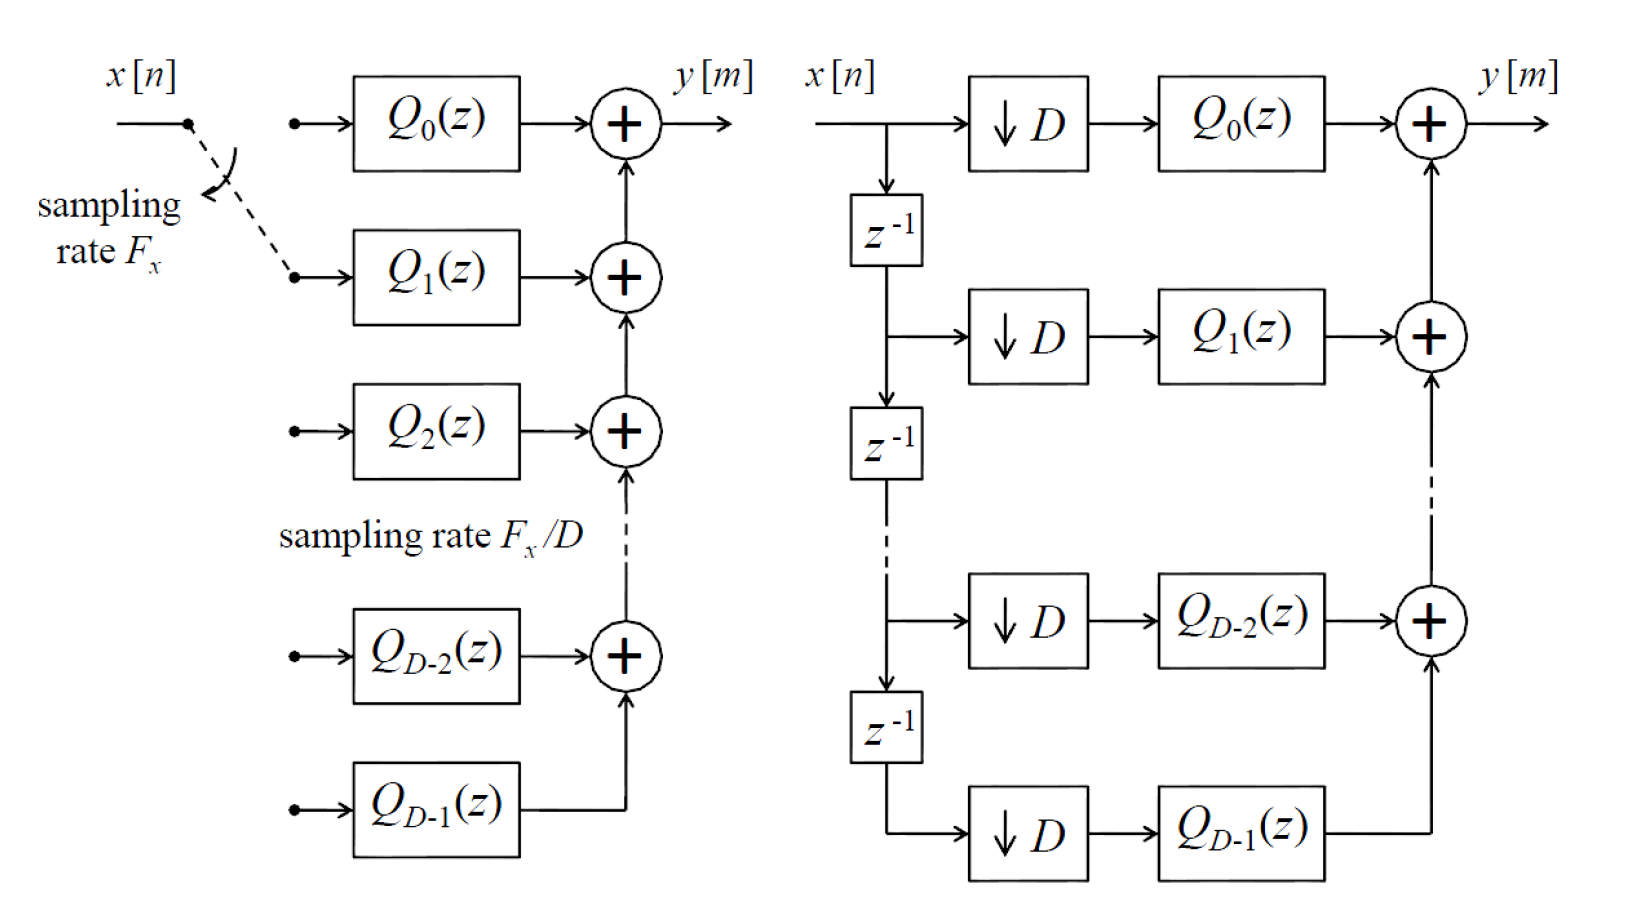
\includegraphics[width=\textwidth]{./images/polyphase_down}
\end{minipage}

%===============================================================================
\section{Abtastrate Realisierung}
Wenn ein up- bzw. downsample Faktor gefordert ist, welcher nicht ganzzahlig ist,
kann dieser mit
\[ \frac{I}{D} \]
dargestellt werden.\\
Wenn zuerst der Downsampler kommt, gehen Informationen verloren. Andersrum
entsteht eine hohe Abtastfrequenz dazwischen. Es ist jedoch vorzuziehen,
zuerst Upsemplen, danach Downsamplen. So kann der Tiefpass der Interpolation
mit dem Tiefpass der Decimation kombiniert werden.
\begin{center}
	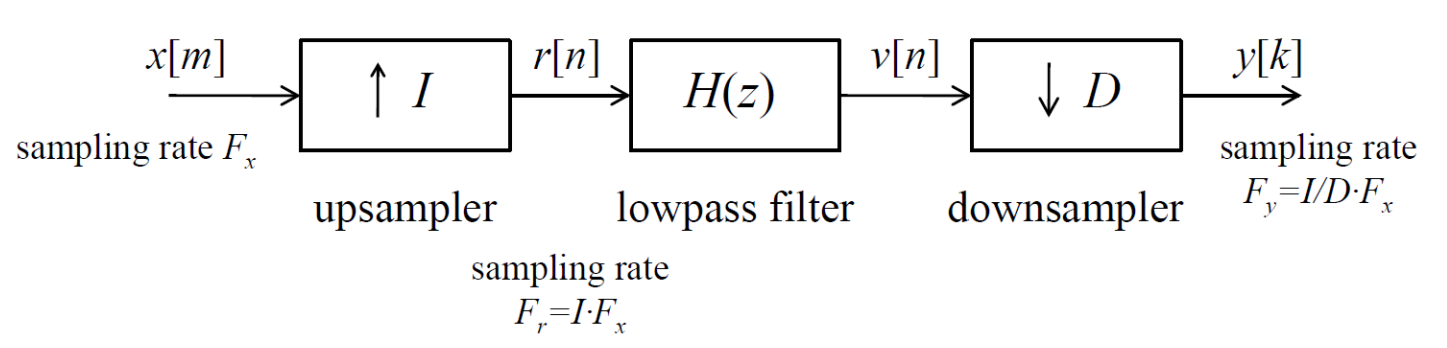
\includegraphics[scale=.7]{./images/sampling}
\end{center}

%===============================================================================
\section{Quadratur Spiegel Filter}
Um den Datenverlust beim Downsampeln zu kompensieren, kann das Signal über zwei
Kanäle übertragen werden. Der eine Kanal filtert das Signal mit einem TP $H_0$,
der Andere mit einem HP $H_1$.
\begin{center}
	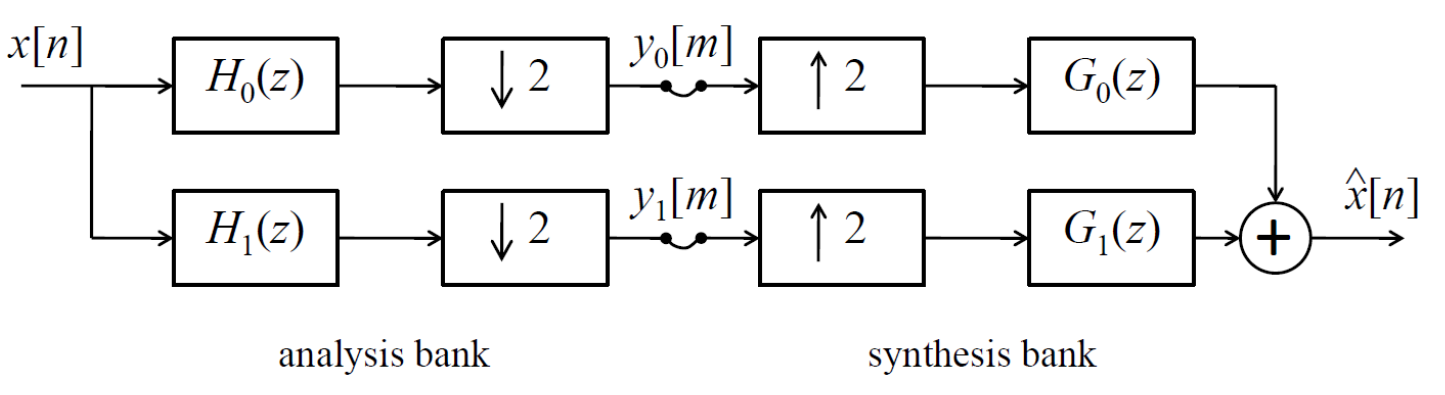
\includegraphics[scale=.7]{./images/quadrature_mirror}
\end{center}
Die DTFT der zwei generierten Signalen $y_0[m]$ und $y_1[m]$ sind:
\[ Y_{0/1} = \frac{1}{2} \left( H_{0/1}\left( \frac{\Omega}{2} \right)
	X\left( \frac{\Omega}{2} \right) + H_{0/1}\left( \frac{\Omega}{2} - \pi
	\right) X\left( \frac{\Omega}{2} -\pi\right) \right)\]
Das Spektrum des synthetisierten Signals $\hat{x}[n]$ ist
\[\begin{aligned} \hat{X}(\Omega) = &\frac12 \left( H_0(\Omega)G_0(\Omega)
	+ H_1(\Omega)G_1(\Omega) \right) \cdot X(\Omega) \\
	+ &\underbrace{\frac12 \left( H_0(\Omega-\pi)G_0(\Omega)
	+ H_1(\Omega-\pi)G_1(\Omega) \right) \cdot X(\Omega-\pi)}_
	{\textrm{alias term}} \end{aligned}\]
Um keinen Aliasterm zu haben müssen die Bedingungen $G_0(\Omega) = H_1(\Omega
-\pi)$ und $G_1(\Omega) = -H_0(\Omega-\pi)$ erfüllt sein:
\[\begin{aligned}
	H_0(\Omega) &= H(\Omega)\\
	H_1(\Omega) &= H(\Omega-\pi)\\
	G_0(\Omega) &= H(\Omega)\\
	G_1(\Omega) &= -H(\Omega-\pi)
\end{aligned}\]
Weiter gilt
\[ \hat{X}(\Omega) = T(\Omega)X(\Omega) \]
mit
\[ T(\Omega) = \frac{1}{2}(H^2(\Omega) -H^2(\Omega-\pi)) \]
Um perfekte Rekonstruktion zu haben, muss $T(\Omega)$ eine Allpass 
Chrakteristik mit linearer Phasenverschiebung aufzeigen. Dies kann am besten
mit einem symetrischen FIR Filter erreicht werden. 
\begin{center}
	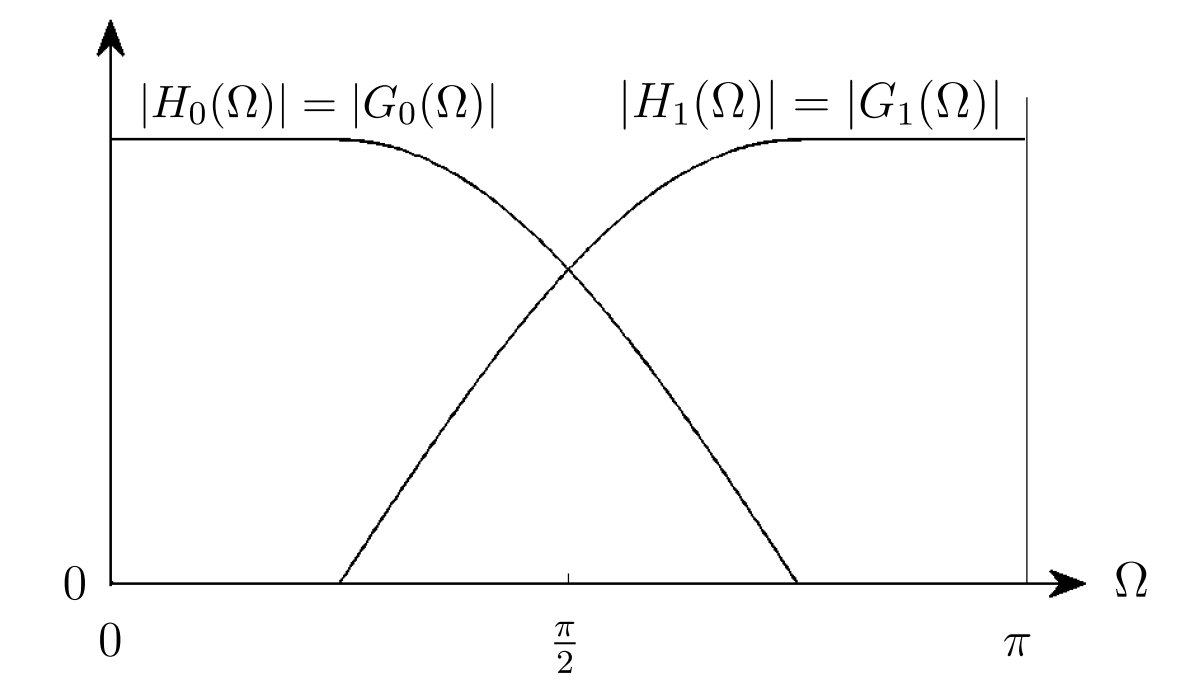
\includegraphics[scale=.7]{./images/power_symetric}
\end{center}
\begin{center}
	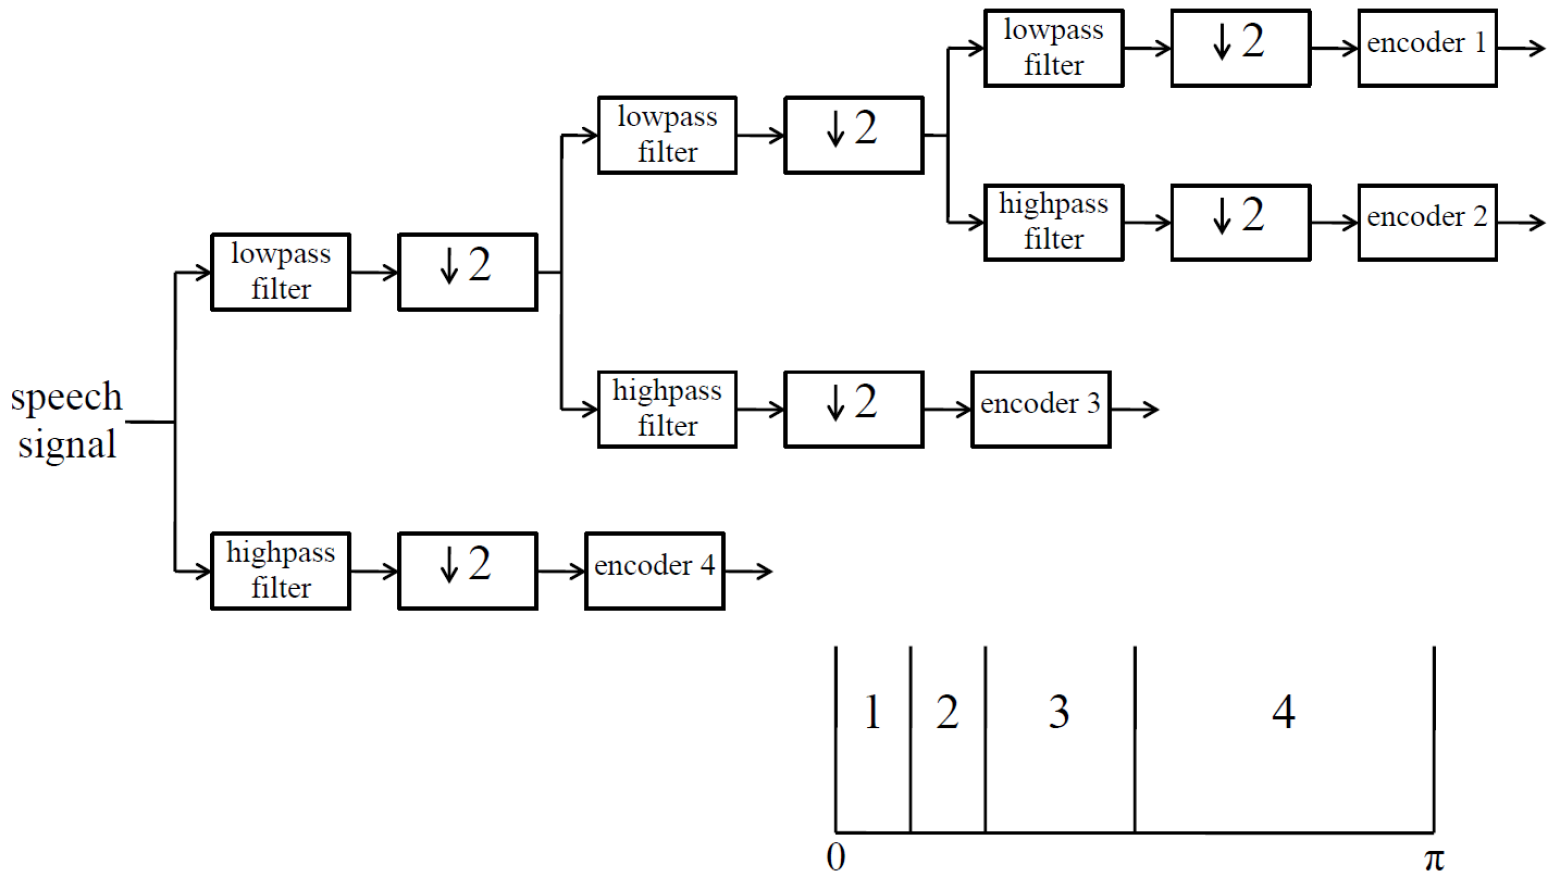
\includegraphics[scale=.7]{./images/quadrature_mirror_ex}
\end{center}

%===============================================================================
\section{DFT Filterbank}
\textbf{critical sampling:} Die Anzahl der Filter $H_0(z), H_1(z), \ldots, H_
{M-1}$ entspricht dem Downsampling $M$.\\
\textbf{oversampling:} Anzahl Kanäle ist grösser als der Downsampling Faktor.\\
\textbf{undersampling:} Anzahl Kanäle ist kleiner als der Downsampling Faktor.\\
\\
\begin{center}
	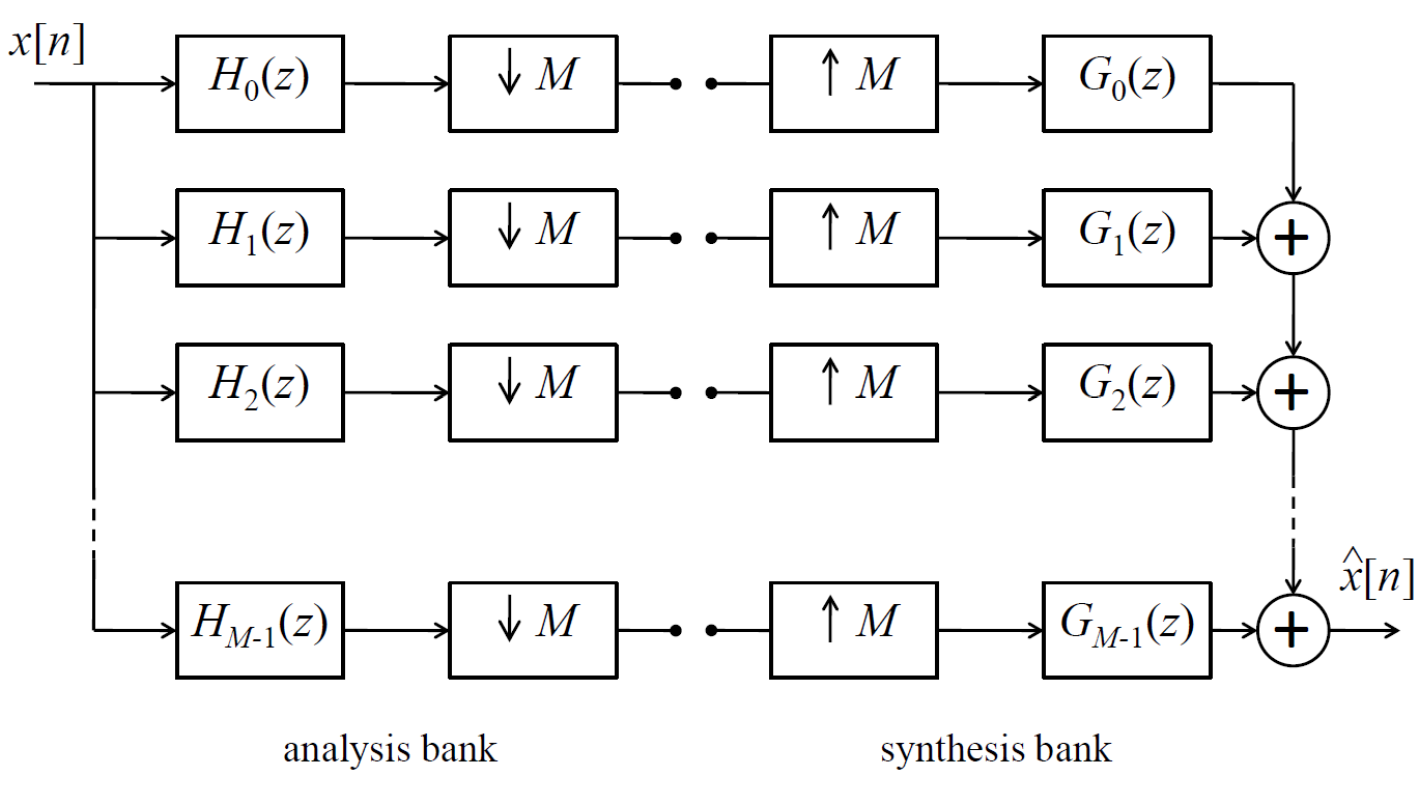
\includegraphics[scale=.7]{./images/critical_sampled}
\end{center}
Prototype Filter $H(z)$:
\[ H_l(z) = H(z\cdot\e^{-\im 2\pi l/M}) \qquad l=0,1,\ldots,M-1 \]
\[ G_l(z) = G(z\cdot\e^{-\im 2\pi l/M}) \qquad l=0,1,\ldots,M-1 \]
Frequenzgang:
\[ H_l(\Omega) = H(\Omega-2\pi l/M) \]
Impulsantwort:\\
\begin{minipage}{.5\textwidth}
	\[ h[k] = \left\lbrace\begin{matrix}
		1	& \textrm{if } k \in \{0,1,\ldots,M-1\}\\
		0	& \textrm{otherwise}
	\end{matrix}\right. \]
\end{minipage}
\begin{minipage}{.5\textwidth}
	\[ g[k] = \left\lbrace\begin{matrix}
		\frac{1}{M}	& \textrm{if } k \in \{0,1,\ldots,M-1\}\\
		0	& \textrm{otherwise}
	\end{matrix}\right. \]
\end{minipage}
Mit polyphase
\[ H_l(z) = \sum_{i=0}^{M-1}\e^{\im 2\pi li/M} \cdot z^{-i} P_i(z^M) 
	\qquad l=0,1,\ldots,M-1 \]
\begin{minipage}{.6\textwidth}
	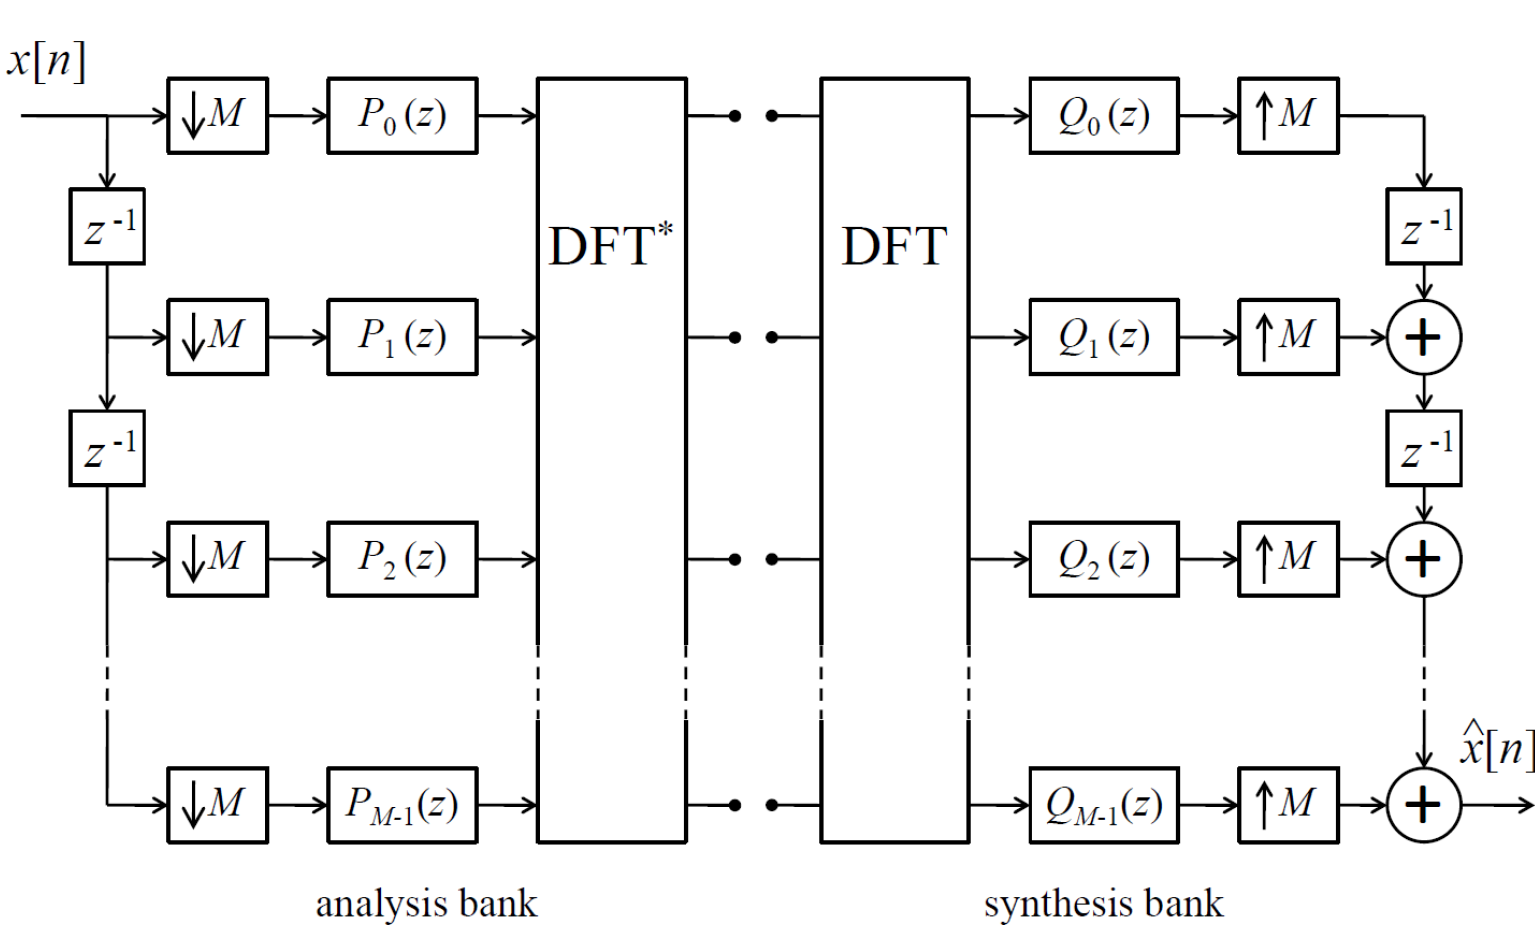
\includegraphics[width=\textwidth]{./images/dft_filterbank}
\end{minipage}
\begin{minipage}{.4\textwidth}
	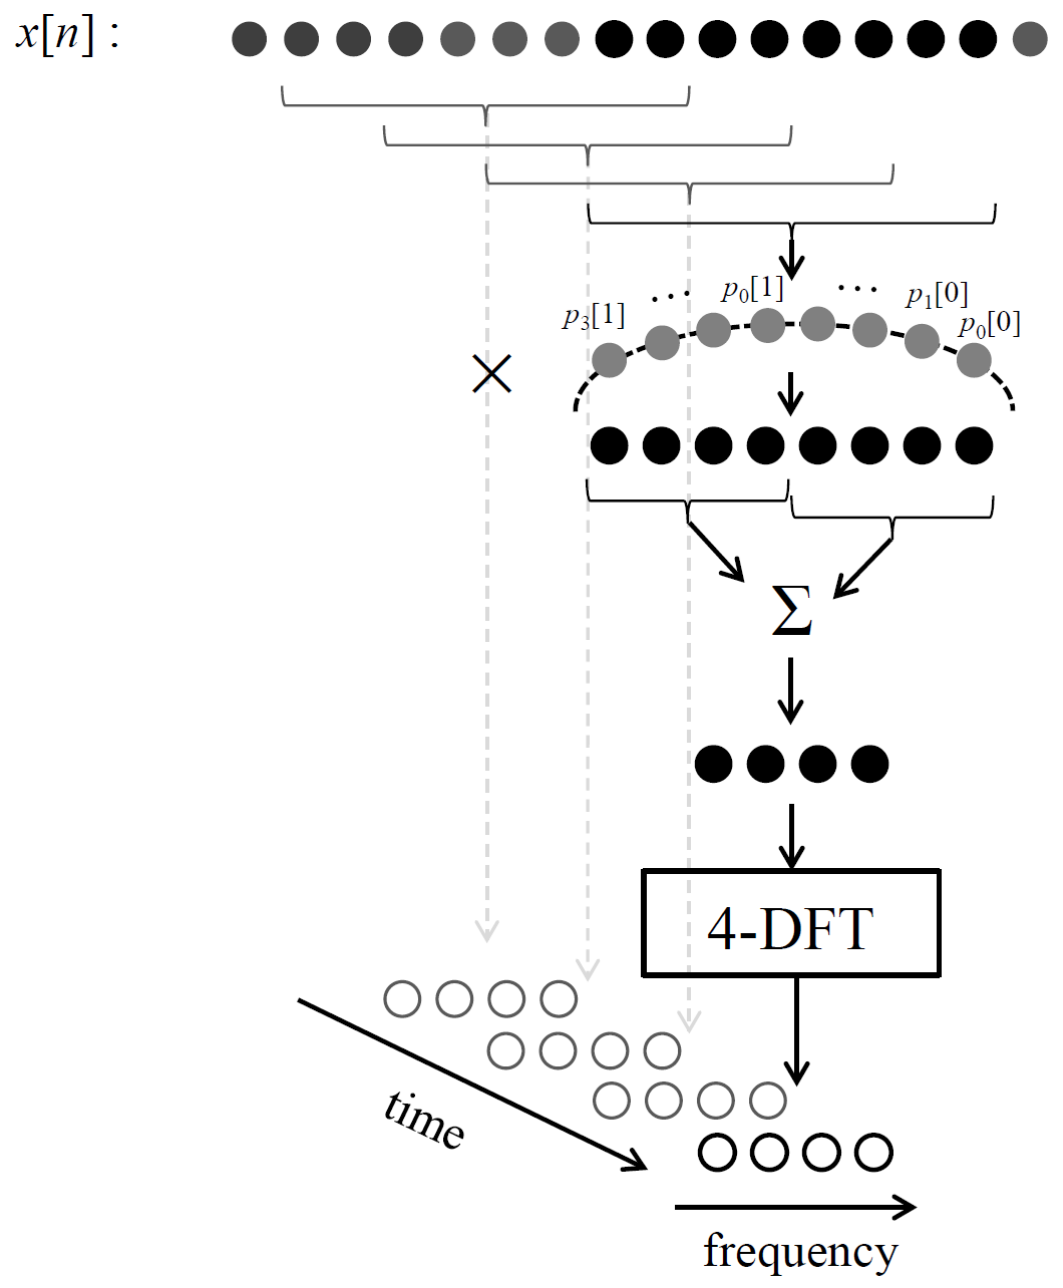
\includegraphics[width=\textwidth]{./images/dft_filter_ill}
\end{minipage}